\documentclass[]{article}
\usepackage{graphicx}
\usepackage{tikz}
\usetikzlibrary{positioning}
\usetikzlibrary{arrows}
\usetikzlibrary{decorations.pathreplacing}
\usepackage[hidelinks]{hyperref}
\usepackage{bbm}
\usepackage{graphicx}
\usepackage{xcolor} % For color
\usepackage{subcaption}
\usepackage{booktabs}
\usepackage{amsmath}
\usepackage{amsfonts}
\usepackage{amssymb}
\usepackage{enumitem}
%\usepackage{enumerate} % For lettered enumeration
\usepackage{amsthm}

%  Make theorems look nice
\newtheoremstyle{mattstyle}%                % Name
{}%                                     % Space above
{}%                                     % Space below
{\itshape}%                                     % Body font
{}%                                     % Indent amount
{\bfseries}%                            % Theorem head font
{.}%                                    % Punctuation after theorem head
{ }%                                    % Space after theorem head, ' ', or \newline
{\thmname{#1}\thmnumber{ #2}\thmnote{ (#3)}}%      

%  State and prove theorems
\theoremstyle{mattstyle}
\newtheorem{theorem}{Theorem}[section]

%  Definitions
\theoremstyle{definition}
\newtheorem{definition}{Definition}[section]

\begin{document}

\title{Machine Learning Notes}
\author{Matthew Scicluna}
\maketitle

\newpage

\tableofcontents

\newpage

\section{Notation}

	\begin{center}		
		\begin{tabular}{*2l}   
			\toprule
			Notation & Meaning
			\\\midrule
			$X$ & random variable \\
			$x$ & instantiation of random variable\\
			$\int f(x) d\mu(x)$ & Lebesgue integral of $f$ w.r.t. measure $\mu$\\
			$\mathbb{R}$ & Set of real numbers\\
			$\mathbb{R}^n$ & Set of $n$-tuples of real numbers\\
			$\mathbb{R}^{n\times m}$ & Set of $n$ by $m$ matrices of real numbers\\
			$\sup(A)$ & Supremum of a set $A$ \\
			$\inf(A)$ & Infemum of a set $A$ \\
			$\mathbbm{1}_{A}(x)$ & Indicator function of set $A$ \\
			$\mathbb{E}_{X\sim p}\{f(X)\}$ & The expected value of $f(X)$ where $X\sim p$\\
			$\mathbb{E}\{X|Y\}$ & The expected value of $X$ conditioned on $Y$ \\
			$\mathcal{Y}^\mathcal{X}$ & the set of functions $f: \mathcal{X}\mapsto \mathcal{Y}$\\
			$\frac{\partial f}{\partial x_i}$ & partial derivative of $f$ w.r.t component $x_i$\\
			$\nabla_{x} f(x)$ & gradient of $f$ evaluated at $x$\\
			$Hf(x)$ & Hessian of $f$ evaluated at $x$\\
			$Jf(x)$ & Jacobian Matrix of $f$ evaluated at $x$\\
			$[A]_{ij}$ & $i$th row and $j$th column of matrix $A$ \\
			$B_r(x)$ & Ball of radius $r$ centred at $x$ \\
			int($A$) & Interior points of set $A$ \\
			bd($A$) & Boundary points of set $A$
			\\\bottomrule
			\hline
		\end{tabular}
	\end{center}

\newpage

\section{Preliminaries}

\subsection{Vector Calculus}

Let $S \subseteq \mathbb{R}^n$ and $x_0$ an interior point of $S$ with $B_r(x_0) \subseteq S$. Given a function $f: S \rightarrow \mathbb{R}^m$ we say that $f$ is \textbf{Differentiable} at $x_0$ if there exists an $A \in \mathbb{R}^{m \times n}$ depending only on $x_0$ s.t. $\forall ||\Delta|| < r$
\begin{align*}
&f(x_0 + \Delta) - f(x_0) = A(x_0)\Delta + r_{x_0}(\Delta)\\
&\text{where $\frac{r_{x_0}(\Delta)}{||\Delta||}\rightarrow 0$ as $\Delta \rightarrow 0$}
\end{align*}

If $f$ is differentiable at every point of an open subset $E$ of $S$, then $f$ is \textbf{Differentiable} on $E$. We call $df(x_0, \Delta) = A(x_0)\Delta \in \mathbb{R}^{m \times 1}$ the first \textbf{Differential} of $f$ at $x_0$.

\begin{theorem}
	$f$ is \textbf{Differentiable} at $x_0$ if and only if each component of f denoted as $f_i$ $i=1,\cdots, m$ is differentiable at $x_0$. In that case $[df(x_0, \Delta)]_i = df_i(x_0, \Delta)$
\end{theorem}
\begin{proof}
	Magnus and Neudecker chapter 5 \cite{magnus1988matrix}
\end{proof}

So $f$ is only differentiable if each of its $m$ components are seperately differentiable. Let $f_i$ be the $i$th component of $f$, with $f$ and $x_0$ defined as before, $e_j$ be the $j$th unit vector of $\mathbb{R}^n$ we define the \textbf{Partial Derivative} of $f_i$ w.r.t $x_j$ as
$$
\frac{\partial f_i(x_0)}{\partial x_j} = \lim\limits_{t \rightarrow 0} \frac{f_i(x_0+te_j) - f_i(x_0)}{t}
$$

We define the \textbf{Jacobian Matrix} of $f$ as:
$$ Jf(x_0) =  \begin{bmatrix}
\frac{\partial f_1(x_0)}{\partial x_1} & \dots  & \frac{\partial f_1(x_0)}{\partial x_n} \\
\vdots & \ddots & \vdots \\
\frac{\partial f_m(x_0)}{\partial x_1} & \dots  & \frac{\partial f_m(x_0)}{\partial x_n}
\end{bmatrix}$$

It can be shown that if $f$ is differentiable, then all its partial derivatives exist, although the converse is not true! This is why Theorem 2.1 only holds in one direction. Note that the Jacobian is defined at any point where all the partial derivatives exist, even if $f$ is not differentiable at that point! When the Jacobian is square, we call its determinant the \textbf{Jacobian} of $f$.

\begin{theorem}
	$[A(x_0)]_{ij} = \frac{\partial f_i(x)}{\partial x_j}\Bigr\rvert_{x=x_{0}}$
\end{theorem} 
\begin{proof}
	Magnus and Neudecker chapter 5 theorem 5 \cite{magnus1988matrix}
\end{proof}

By construction, $Jf(x_0) = A(x_0)$. We call the transpose of the Jacobian Matrix the \textbf{Gradient} and denote it as $\nabla_x f(x_0)$. Finally, we give an important result: the chain rule.
\begin{theorem}[Chain Rule]
	Let $f$,$x_0$ defined as before and $g: T \rightarrow \mathbb{R}^p$. Suppose that $T \subseteq \mathbb{R}^m$, $f(S) \subseteq T$, $f(x_0)$ is an interior point of $T$, and that $g$ is differentiable at $f(x_0)$. Then $Jg \circ f(x_0) = Jg(f(x_0))Jf(x_0)$
\end{theorem} 
\begin{proof}
	Magnus and Neudecker chapter 5 theorem 8 \cite{magnus1988matrix}
\end{proof}

As a sanity check, we can see that $Jg \circ f(x_0) \in \mathbb{R}^{p \times n}$ while  $Jg(f(x_0))\in \mathbb{R}^{p \times m}$ and $Jf(x_0)\in \mathbb{R}^{m\times n}$.

\subsubsection{Many to One Functions and the Hessian}

The majority of functions we work with in machine learning are real valued, meaning they are of form $f: \mathbb{R}^n \rightarrow \mathbb{R}$. This is since they are either loss functions or probability densities. Hence we focus on this case. The most common use of vector calculus is to optimize a function by finding its stationary points (where the gradient is 0) and to check whether it is a maxima or minima by checking the Hessian. First we present a simpler version of the chain rule for gradients.
 
\begin{theorem}[Simplified Chain Rule]
If we consider only functions $g$ with $p=1$ then the gradient is: $$\nabla_x g \circ f(x) = Jf(x)^T\nabla_{x}g(f(x))$$
\end{theorem} 

The Jacobian matrix for $f$ takes the following form: 
$$J f(x) = \left(\frac{\partial f}{\partial x_1}, \cdots, \frac{\partial f}{\partial x_n}\right) \in \mathbb{R}^{1 \times n}$$
The Gradient for $f$ is then: 
$$\nabla_{x} f(x) = \left(\frac{\partial f}{\partial x_1}, \cdots, \frac{\partial f}{\partial x_n}\right)^T \in \mathbb{R}^{n \times 1}$$

We define the \textbf{Second Partial Derivative} for a real valued $f$ as follows. Let $f$, $e_i$ as before. The second partial derivative of $f$ w.r.t $x_i$ and $x_j$ is:
$$
\frac{\partial^2 f(x_0)}{\partial x_i \partial x_j} = 
\lim\limits_{t \rightarrow 0} \frac{ \frac{\partial f(x_0+te_i)}{\partial x_j} - \frac{\partial f(x_0)}{\partial x_j} }{t}
$$

We define the \textbf{Hessian} for real valued functions as: 
$$H f(x_0) = \begin{bmatrix}
\frac{\partial^2 f(x_0)}{\partial x_1^2} & \dots  & \frac{\partial^2 f(x_0)}{\partial x_n \partial x_1} \\
\vdots & \ddots & \vdots \\
\frac{\partial^2 f(x_0)}{\partial x_1 \partial x_n} & \dots  & \frac{\partial^2 f(x_0)}{\partial x_n^2}
\end{bmatrix}\in \mathbb{R}^{n \times n}$$

\newpage

\subsubsection{Some Important Examples}

We now get to the payoff, some important results which will appear often in these notes. Let $b \in \mathbb{R}^n$, $B \in \mathbb{R}^{n \times n}$

\begin{theorem}
	$\nabla_{x} x^TBx = x^T(B^T+B)$
\end{theorem}
\begin{proof}
	Notice 
	\begin{align*}
	(x+\Delta)^TB(x+\Delta) - x^TBx &= \Delta^TBx + x^TB\Delta + \Delta^TB\Delta\\
	&= x^T(B + B^T)\Delta + \Delta^TB\Delta\\
	&= A(x)\Delta + r_{x}(\Delta)\\
	\end{align*}
	Where $r_{x}=\Delta^TB\Delta$ and $A(x)=x^T(B + B^T)$. We see that $r_{x}\in O(||\Delta||)$, and so the differential is $x^T(B + B^T)\Delta$. Therefore, $\nabla_x x^TBx = (B + B^T)x$, the transpose.
\end{proof}

\begin{theorem}
	$\nabla_{\mu} (x-b)^TB(x-b) = (x-b)^T(B+B^T)$
\end{theorem}
\begin{proof}
	We use the chain rule where $f(x)=x-b$ and $g(y)=y^TBy$.
	\begin{align*}
	&\nabla_{y}g(y) = (B + B^T)y\\
	&Jf(x) = I \\
	&\nabla_{x} g \circ f(x) = (B + B^T)(x-b)
	\end{align*}
\end{proof}

For the final example, we must refine our definition of differentiability to include matrices. That's right, you can actually do that. First we define the norm of a matrix $A$ as:
$$ ||A|| = tr(A^TA)^{\frac{1}{2}} $$

Let $S \subseteq \mathbb{R}^{n \times m}$ and $x_0$ an interior point of $S$ with $B_r(x_0) \subseteq S$. Given a function $f: S \rightarrow \mathbb{R}$ we say that $f$ is \textbf{Differentiable} at $x_0$ if there exists an $A \in \mathbb{R}^{n \times m}$ depending only on $x_0$ s.t. $\forall ||\Delta|| < r$
\begin{align*}
&f(x_0 + \Delta) - f(x_0) = tr(A(x_0)^T\Delta) + r_{x_0}(\Delta)\\
&\text{where $\frac{r_{x_0}(\Delta)}{||\Delta||}\rightarrow 0$ as $\Delta \rightarrow 0$}
\end{align*}

We define the Jacobian and Gradient in terms of $A(x_0)$ in the same way that we did for vector valued functions.

\newpage

\begin{theorem}
	$\nabla_{B} \log \det B = B^{-1}$ for $B$ symmetric, invertible
\end{theorem}
\begin{proof}
	First notice the following decomposition
\begin{align*}
\log \det (B + \Delta) &= \log \det\left(B^{\frac{1}{2}}\left(I + B^{-\frac{1}{2}}\Delta B^{-\frac{1}{2}}\right)B^{\frac{1}{2}}\right)\\
&= \log\left(\det\left( B^{\frac{1}{2}}\right) \det\left(I + B^{-\frac{1}{2}}\Delta B^{-\frac{1}{2}}\right) \det\left(B^{\frac{1}{2}}\right) \right)\\
&=\log\det\left(I + B^{-\frac{1}{2}}\Delta B^{-\frac{1}{2}}\right)+\log\det B
\end{align*}

We try to find our differential in the same way we did in the first example:
\begin{align*}
\log \det (B + \Delta) - \log\det B &= \log\det\left(I + B^{-\frac{1}{2}}\Delta B^{-\frac{1}{2}}\right)\\
&\overset{(a)}{=} \sum_{i} \log\left(1 + \lambda\left(B^{-\frac{1}{2}}\Delta B^{-\frac{1}{2}}\right)\right)\\
&\overset{(b)}{=} \sum_{i}\lambda\left(B^{-\frac{1}{2}}\Delta B^{-\frac{1}{2}}\right) + O(||\Delta||)\\
&\overset{(c)}{=} \text{tr}\left(B^{-\frac{1}{2}}\Delta B^{-\frac{1}{2}}\right) + O(||\Delta||)\\
&= \text{tr}(B^{-1}\Delta) + O(||\Delta||)
\end{align*}
Where (a) follows since $\det A = \prod_i \lambda_i(A)$; (b) using $\log(1+x)=x+O(x^2)$ for $|x|<1$; and (c) using tr($A$)$=\sum_i \lambda_i(A)$. 
We use the characterization of the gradient for functions of matrices to get that $\nabla_B \log\det B = B^{-1}$.
\end{proof}

Finally, we mention in passing some other useful identities.
\begin{itemize}
	\item $\nabla_{x} b^Tx = \nabla_{x} x^Tb= b$
	\item $\nabla_{B} x^TBx = xx^T$
\end{itemize}

\newpage

\subsection{Optimization}\label{sec:optim}

We now discuss how to solve optimization problems. We want to minimize our \textbf{Objective Function} $f_0 : \mathbb{R}^n \rightarrow \mathbb{R}$ w.r.t some  \textbf{Optimization Variable} $x \in \mathbb{R}^n$ subject to some \textbf{Inequality Constraints} $f_i: \mathbb{R}^n \rightarrow \mathbb{R}$ and some \textbf{Equality Constraints} $h_i: \mathbb{R}^n \rightarrow \mathbb{R}$. If there are no constraints (i.e.) $m=p=0$ then we call the problem \textbf{Unconstrained}. We set $f_0(x) = \infty$ for $x \notin$dom($f_0$).
Formally, our optimization problem can be written as:
\begin{align*}
\text{Minimize } & f_0(x) \\
\text{subject to } & f_i(x) \le 0 \ i = 1, \cdots, m\\
& h_i(x) = 0 \ i = 1, \cdots, p
\end{align*}

We denote the intersection of the domains of $f_0$, the $f_i$'s and the $h_i$'s as $\mathcal{D}$. We call a point $x$ \textbf{Feasible} if $x\in \mathcal{D}$ and $x$ satisfies the constraints. The \textbf{Optimal Value} of this problem is $p^*=\inf\{f_0(x): \text{x feasible}\}$. If $x$ feasible and $f_0(x) = p^*$ then we call it an \textbf{Optimal Point}. The set of Optimal Points is called the \textbf{Optimal Set}. Often we will find points which minimize $f_0$ only over points within some radius. Such points are called \textbf{Locally Optimal}.
We note two degenerate cases to be careful for:
\begin{itemize}
	\item the problem has no feasible points, so we set $p^*=\infty$
	\item the problem has arbitrarily small optimal values, $p^*=-\infty$
\end{itemize}

\subsubsection{Convex Sets and Functions}

We describe a highly desirable property of functions we are optimizing over: Convexity. If a function is convex then any locally optimal point is globally optimal.
A set $A$ is called \textbf{Convex} if:
\begin{align*}
(1-\alpha)x + \alpha y \in A \\
\forall x,y\in A \text{ and } \forall\alpha \in [0,1]
\end{align*} 
A function $f$ is \textbf{Convex} if:
\begin{align*}
f((1-\alpha)x + \alpha y) \le (1-\alpha)f(x) + \alpha f(y)\\
\forall x,y\in \text{dom(f)}\text{ and } \forall\alpha \in [0,1]
\end{align*} 

If the equality is strict (i.e. $<$) then $f$ is called \textbf{Strictly Convex}. We call a function \textbf{Concave} if $-f$ is convex. There is a relationship between convexity of a set and that of a function. We define the \textbf{Epigraph} of a function is as:
$$\Bigl\{ (x,t): x\in \text{dom(f)}, t\ge f(x) \Bigr\}$$
\begin{theorem}
	A function $f$ is convex if and only if its epigraph is a convex set
\end{theorem}
\begin{proof}
	Boyd \cite{Boyd:2004:CO:993483} 
\end{proof}
\newpage

We present some examples of Convex functions.
\begin{itemize}
	\item $\exp{ax}, -\log x$
	\item Any norm over $\mathbb{R}^n$
	\item non-negative weighted sums of convex functions $f_i$'s
	\item Let $f$ be convex with domain $\mathcal{X} \times \mathcal{Y}$. If for each $y \in \mathcal{Y}$ we have that $f(x,y)$ is convex in $x$; then $$ g(x) = \sup_{y \in \mathcal{Y}} f(x,y) \ \text{is convex in $x$}$$
\end{itemize}

To check for convexity, we present first and second order conditions which are both necessary and sufficient:
\begin{theorem}
	A function $f$ is convex if and only if dom($f$) is convex and $\forall x,y \in$dom($f$)
	$$ f(y) \ge f(x) + \nabla f(x)^T(y-x)$$
\end{theorem}
\begin{proof}
	Boyd section 3.1.3 \cite{Boyd:2004:CO:993483} 
\end{proof}
This is a significant result since this demonstrates how local information from a convex function (i.e. its derivative) can yield global information about it (the inequality holds across its entire domain)!

\begin{theorem}
	A function $f$ is convex if and only if dom($f$) is convex and $\forall x \in$dom($f$) $Hf(x)$ is positive semi definite.
\end{theorem}
\begin{proof}
	Boyd section 3.1.4 \cite{Boyd:2004:CO:993483} 
\end{proof}

We can strengthen the result. If dom($f$) is convex and $Hf(x)$ is positive definite, then $f$ is strictly convex. The converse, however, does not hold. A \textbf{Convex Optimization Problem} is an optimization problem where $f_0, f_1, \cdots, f_m$ are convex and $h_i$ are \textbf{Affine}: $h(x) = 0$ can be written as $Ax = b$, where $A \in \mathbb{R}^{d \times n}$, $b\in\mathbb{R}^n$. These problems have a very appealing property: 
\begin{theorem}
	For any convex optimization problem, any locally optimal point is optimal.
\end{theorem}
\begin{proof}
	Boyd section 4.2.2 \cite{Boyd:2004:CO:993483} 
\end{proof}

\subsubsection{Unconstrained Optimization}

For unconstrained problems it is easy to verify whether a point is a local optima as these points have clear first and second order necessary and sufficent conditions. If $x^*$ is a local minima of $f_0$ and $f_0$ is twice continuously differentiable and $x^* \in$int($\mathcal{D}$); then the following are necessary:
$\nabla_{x}f_0(x^*)=0$ and $Hf_{0}(x^*)$ positive semi-definite. The following are sufficient: $\nabla_{x}f_0(x^*)=0$ and $Hf_{0}(x^*)$ is positive definite.

If $f_0$ is convex then the local minima is the optimal point. If $f_0$ is not convex the procedure becomes more complicated. We must compare the points satisfying the sufficient conditions (or just the necessary ones if none satisfy the sufficient ones) along with any points in bd($\mathcal{D}$) to find the minima.

\subsubsection{Langrangian Duality}
We can solve our optimization problem using the \textbf{Lagrangian} $L: \mathbb{R}^n\times \mathbb{R}^m\times \mathbb{R}^p \rightarrow \mathbb{R} $ with domain $\mathcal{D}\times\mathbb{R}^m\times \mathbb{R}^p$
\begin{equation}\label{eq:primal}
L(x,\lambda,\nu) = f_0(x) + \sum_{i=1}^m \lambda_if_i(x) + \sum_{i=1}^p \nu_i h_i(x)
\end{equation}

The Langrangian itself may be difficult to minimize. The problem can be simplified by introducing the \textbf{Lagrange dual function} $g: \mathbb{R}^m\times \mathbb{R}^p \rightarrow \mathbb{R}$
\begin{equation}\label{eq:dual}
g(\lambda,\nu) =\inf\limits_{x\in D} L(x,\lambda,\nu)
\end{equation}

We call (\ref{eq:primal}) the \textbf{Primal Problem} and (\ref{eq:dual}) the \textbf{Dual Problem}. We note that $g$ is concave (regardless of $f_0$) and can be $-\infty$. We call $(\lambda, \nu)$ \textbf{Dual Feasible} if $\lambda \ge 0$ and $(\lambda, \nu) \in$ dom($g$), where dom($g$)=$\{ (\lambda, \nu) | g(\lambda, \nu)>-\infty\}$ \footnote{We note that we could add extra constraints to prevent $g(\lambda, \nu)=-\infty$ and this would not change anything. See Boyd section 5.2.1 \cite{Boyd:2004:CO:993483}}. We denote $d^*$ as the \textbf{Dual Optimum Value}: the infemum of $g$. We say that $(\lambda,\nu)$ is \textbf{Dual Optimum} if it is dual feasible and $g(\lambda,\nu)=d^*$. We now relate the primal and dual problems:
\begin{theorem}[Lower Bound Property]
	Let $\lambda \ge 0$, then $g(\lambda, \nu) \le p^*$ 
\end{theorem}
\begin{proof}
	Note that for any feasible $\tilde{x}$ and $\lambda \ge 0$:
	$$f_0(\tilde{x}) \ge L(\tilde{x}, \lambda, \nu) \ge \inf\limits_{x\in D} L(x,\lambda,\nu) = g(\lambda, \nu)$$
	and since $p^*$ is the infemum of all feasible $\tilde{x}$, it follows that $ p^* \ge g(\lambda, \nu)$
\end{proof}

Instead of minimizing $f_0$ using the primal we can maximize the lower bound $g$. This may be an easier problem since $g$ is always concave. It is clear that we always have \textbf{Weak Duality} $p^* \ge d^*$, although we want \textbf{Strong Duality}: $p^* = d^*$. A sufficient condition for strong duality is \textbf{Slater's Condition}.

\begin{theorem}[Slater's Condition]
	Suppose we have a convex primal, and that int($\mathcal{D}$) is non empty. If $\exists x \in$int($\mathcal{D}$) satisfying $f_1(x)<0, \cdots, f_m(x)<0$ and $h_1(x)=0, \cdots, h_p(x)=0$, we have strong duality. If any $f_i$ are affine, we only need them to satisfy $f_i(x)=0$.
\end{theorem}
\begin{proof}
	Boyd section 5.3.2 \cite{Boyd:2004:CO:993483}
\end{proof}

\subsubsection{Saddle Point Interpretation}

Given a $w^*\in W$, $z^*\in Z$ we say that $(w^*,z^*)$ is a \textbf{Saddle Point} for function $f$ with domain $W \times Z$ if $f(w^*, z) \le f(w^*, z^*) \le f(w, z^*)$ for all $(w,z) \in W \times Z$. This means that $w^*$ minimizes $f(w, z^*)$ over $W$ and $z^*$ maximizes $f(w^*, z)$ over $Z$:
\begin{align*}
f(w^*, z^*) = \inf_{w \in W} f(w, z^*) = \sup_{z \in Z} f(w^*, z)
\end{align*}

First we notice the following:
\begin{align*}
\sup\limits_{\substack{\lambda\ge0 \\ \nu}} L(x, \lambda, \nu) &= \sup\limits_{\substack{\lambda\ge0 \\ \nu}} \left( f_0(x) + \sum_{i=1}^m \lambda_if_i(x) + \sum_{i=1}^p \nu_i h_i(x) \right)\\
&= \begin{cases}
f_0(x) & \text{$x$ is feasible}\\
\infty & \text{o.w.}
\end{cases}
\end{align*}

We can show this in cases. Suppose $x$ is feasible. $h_i(x)=0$ so we can ignore them. Since $f_i(x) \le 0,\ i=1, \cdots, m$; $\lambda = 0$ would optimize $L$ since $\sum_{i=1}^m \lambda_if_i(x) \le 0$. Now suppose $x$ was infeasible and WLOG suppose that $ \exists j \ s.t.\ f_j(x) > 0$, then we can make $L$ arbitrarily large by taking $\lambda_j \rightarrow \infty$. The same reasoning works for any $h_i(x) \ne 0$. Hence the result. From this we can express $p^*$ as:
\begin{align*}
p^* &= \inf_x f_0(x), \text{  x feasible}\\
&= \inf_x\sup_{\substack{\lambda\ge0 \\ \nu}}L(x, \lambda, \nu)
\end{align*}

and our dual is defined as
\begin{align*}
d^* = \sup_{\substack{\lambda\ge0 \\ \nu}}\inf_x L(x, \lambda, \nu)
\end{align*}

Hence strong duality can be expressed in the following way, clearly showing that $(x, \lambda, \nu)$ is a saddle point for $L$.
\begin{align*}
\inf_x\sup_{\substack{\lambda\ge0 \\ \nu}}L(x, \lambda, \nu) = \sup_{\substack{\lambda\ge0 \\ \nu}}\inf_x L(x, \lambda, \nu)
\end{align*}

\newpage

\subsubsection{KKT Conditions}

We now state some conditions often used to determine whether a solution $x^*$ of $f$ is optimal. These are the \textbf{KKT Conditions}.

\begin{theorem}[KKT Conditions]
	Let $f_0, f_i, h_i$ be differentiable (and so they have open domains). If $x^*$ is optimal and $(\lambda^*, \nu^*)$ are dual optimal and we have strong duality; then the following Conditions must be satisfied:
	\begin{itemize}
		\item $\nabla_x f_0(x^*) + \sum_{i=1}^m \lambda_i^* \nabla_x f_i(x^*) + \sum_{i=1}^p \nu_i^* \nabla_x h_i(x^*) = 0$ $\rightarrow$ Stationarity
		\item $\lambda_i^* f_i(x^*)=0 \rightarrow$ Complementary Slackness
		\item $x^*$ is feasible $\rightarrow$ Primal Feasibility
		\item $\lambda^* \ge 0 \rightarrow$ Dual Feasibility
	\end{itemize}
\end{theorem}
\begin{proof}
	We have to show Stationarity and Complementary Slackness. Notice that
	\begin{align}
	f_{0}(x^*) = g(\lambda^*, \nu^*) &= \inf_x \left( f_0(x) + \sum_{i=1}^m \lambda_i^*f_i(x) + \sum_{i=1}^p \nu_i^* h_i(x) \right) \\
	&\le f_0(x^*) + \sum_{i=1}^m \lambda_i^*f_i(x^*) + \sum_{i=1}^p \nu_i^* h_i(x^*)\\
	&\overset{(a)}{\le} f_0(x^*)
	\end{align}
	Where (a) comes from the condition that $h_i(x^*) = 0 \Rightarrow \sum_{i=1}^p \nu_i^* h_i(x^*) = 0$ and $f_i(x^*) \le 0, \lambda_i \ge 0 \Rightarrow \sum_{i=1}^m \lambda_i^* f_i(x^*) \le 0$. We get that $\inf\limits_{x} L(x, \lambda^*, \nu^*) = f_0(x^*)$, i.e. $x^*$ minimizes $L(x, \lambda^*, \nu^*)$ which implies Stationarity. Complementary slackness comes from $\sum_{i=1}^m \lambda_i^* f_i(x^*) = 0$ and $\lambda_i^* f_i(x^*) \le 0 \Rightarrow \lambda_i^* f_i(x^*) = 0$ for every $i$.
\end{proof}

\begin{theorem}
	If $x^*, \lambda^*, \nu^*$ satisfy the KKT conditions and the primal is convex; then $x^*$ is optimal, $\lambda^*, \nu^*$ are dual optimal and we have strong duality.
\end{theorem}
\begin{proof}
	\begin{align}
	g(\lambda^*, \nu^*) &= \inf_x \left( f_0(x) + \sum_{i=1}^m \lambda_i^*f_i(x) + \sum_{i=1}^p \nu_i^* h_i(x) \right) \\
	&\overset{(a)}{=}f_0(x^*) + \sum_{i=1}^m \lambda_i^*f_i(x^*) + \sum_{i=1}^p \nu_i^* h_i(x^*)\\
	&\overset{(b)}{=}f_0(x^*)
	\end{align}
	Since $\lambda^*\ge0$, $L(x,\lambda^*,\nu^*)$ is convex in $x$. By the KKT conditions, $x^*$ is primal feasible and $\nabla_x L(x,\lambda^*,\nu^*)$ evaluated at $x^*$ is 0 $\Rightarrow$ $x^*$ minimizes $L(x,\lambda^*,\nu^*)$ (a). (b) follows from complementary slackness. Therefore, we have strong duality and so $x^*$ is optimal and $\lambda^*, \nu^*$ are dual optimal.
\end{proof}

%So the KKT conditions are necessary for optimality where $f_0,f_i,h_i$ are %differentiable and there is strong duality. Likewise, if $L$ is convex and %$x^*,\lambda^*,\nu^*$ satisfy KKT, then $x^*$ is optimal, $(\lambda^*,\nu^*)$ are %dual optimal, and there is strong duality.

%\begin{theorem}
%	If Slaters condition is satisfied, then $x^*$ is optimal if and only if there exists $\lambda^*, \nu^*$ such that $(x^*,\lambda^*, \nu^*)$ satisfy KKT conditions.
%\end{theorem}
%\begin{proof}
%	Boyd section 5 \cite{Boyd:2004:CO:993483}
%\end{proof}

%\subsubsection{Finding Optimal Points}

In some cases we can find optimal points by using the Dual to solve the Primal. Specifically; if:
\begin{enumerate}
	\item strong duality holds
	\item $(\lambda^*, \nu^*)$ is a dual optimal solution
	\item $L(x, \lambda^*, \nu^*)$ has a unique minimum value (e.g. $L(x, \lambda^*, \nu^*)$ is strictly convex in $x$)
\end{enumerate}
Let $x^*$ be the unique optima, then either:
\begin{enumerate}
	\item $x^*$ is feasible; and so $x^*$ must be optimal.
	\item $x^*$ is not feasible and no optimal can exist.
\end{enumerate}

\newpage

\subsection{Basic Probability}

We now discuss the requisite probability theory needed for Machine Learning. First, some definitions: \textbf{Probability} quantifies uncertainty of data given a model. Probabilistic questions are usually well-formed mathematical problems. \textbf{Statistics} is the inverse problem: given data, how likely is model? These questions tend to be ill-formed since many models can generate the same data! See figure for a picture of this.

\begin{figure}
	\begin{center}
		\begin{tikzpicture}[scale=2.5]\label
		\node [blue] at (0.75, 0.4) {Probability Theory};
		\node [red] at (0.75, -0.9) {Statistics (ill-defined)};
		\draw [->,ultra thick,blue] (0,0) to [bend left=40] (1.5,0);
		\draw [->,ultra thick,red] (1.5,-0.5) to [bend left=40] (0,-0.5) ;
		\node at (0,-0.2) {\huge{$ \theta $}};
		\node at (1.5,-0.2) {\huge{$ X $}};
		\node at (0,-0.4) {model};
		\node at (1.5,-0.4) {data};
		\end{tikzpicture}
	\end{center}
\end{figure}



We now give the basic notions in probability theory.

\subsubsection{Probability Space}
A \textbf{Probability Space}: a triple \( (\Omega, F, \mu)\) consisting of \( \Omega \) the \textbf{Sample Space}, \( F \subseteq 2^{\Omega}\) a \textbf{\(\sigma\)-algebra} on \(\Omega\)  and a \textbf{Probability Measure} \(\mu\): \(F \mapsto [0,1] \). We can compute Probabilities of Events Conditioned on other Events. We define the \textbf{Conditional Probability} of event \(A\) on event \(B\) with \(\mu(B) > 0\) as:
\begin{align*}
\mu(A \mid B) = \frac{\mu(A \cap B)}{\mu(B)} = \frac{\mu(B \mid A)\mu(A)}{\mu(B)}
\end{align*}

A set of events \(\{A_i\}\) are \textbf{Mutually Independent} if, for any subset of \(\{A_j\}_{j\in k}\):
\begin{align*}
\mu \left( \bigcap_{j\in k} A_j \right) = \prod_{j\in k}\mu(A_j) 
\end{align*}

Finally we have the \textbf{Law of Total Probability}: Given Events \(A\) and \textbf{Partition} \(\{B_i\}\) (i.e. where \(\bigsqcup_{i=1}^{\infty} B_i = \Omega \) )
\begin{align*}
\mu(A) = \sum_{i=1}^{\infty} \mu(A \mid B_i)\mu(B_i)
\end{align*}

\subsubsection{Random Variables and Vectors}

A \textbf{Random Variable} is a \(\mathbb{B}\)-Measurable function  \(X: (\Omega, F) \mapsto (\mathbb{R},\mathbb{B}) \). For \( A \in \mathbb{B}\) we can compute \( \mu(X \in A)\) as:
$$\mu(X \in A) := \mu(X^{-1}(A)) = \mu(\{ \omega \in \Omega : X(\omega) \in A \})$$

Where \( \mu(X^{-1}(\cdot)) := \mu_X(\cdot)\) is called the \textbf{Push-Forward Measure} of \(P\) by \(X\) on \( \mathbb{R}\). Hence \( X\) induces a new Probability Space \((\mathbb{R}, \mathbb{B}, \mu_X) \) from the original \( (\Omega, F, \mu)\)

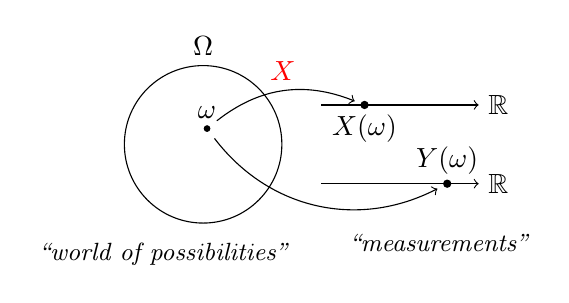
\begin{tikzpicture}[scale=0.5]
%% \draw[help lines] (0,0) grid (12,6);
%% \node [align=center, red] at (1, 1.5) {bla \\ bla} ;
%% \draw [blue, thick] (6,5) rectangle (10,10);
\draw (0,0) circle (2cm);
\node[above] at (0,2) {$\Omega$};
\node (o) at (0.1,.4) {};
\draw (o) circle[radius=2pt] node[above] {$\omega$};
\fill (o) circle[radius=2pt];
\node at (-1,-2.8) {\emph{\small ``world of possibilities''}};

\draw [->] (3,1) -- (7,1) node[right]{$\mathbb{R}$};
\node (x) at (4.1,1) {};
\draw (x) circle[radius=2pt] node[below] {$X(\omega)$};
\fill (x) circle[radius=3pt];
\draw [->, black!70!black] (o) to [bend left=30] node[midway, above, red] {$X$} (x);

\draw [->] (3,-1) -- (7,-1) node[right]{$\mathbb{R}$};
\node (y) at (6.2,-1) {};
\draw (y) circle[radius=2pt] node[above] {$Y(\omega)$};
\fill (y) circle[radius=3pt];
\draw [->, thin] (o) to [bend right=40] (y);
\node at (6,-2.5) {\emph{\small ``measurements''}};
\end{tikzpicture}

Random Variables can be uniquely determined by their \textbf{CDF}:
\( F_X(t) := \mu_X\left((-\infty,t]\right) = \mu(X \le t) \). They always satisfy the folling properties:
\begin{enumerate}
	\item Right Continuous
	\item Non-Negative
	\item \(\lim\limits_{t \to \infty} F_X(t) = 1, \lim\limits_{t \to -\infty} F_X(t) = 0\)
\end{enumerate}
Additionally, any function satisfying above properties is the CDF for some random variable. Random Variables studied are usually either \textbf{Continuous} or \textbf{Discrete} (although they can also be \textbf{Singular} or \textbf{Mixed}).

We say that $F$ is \textbf{Absolutely Continuous} if it is differentiable a.e. and $\exists f(x)$ s.t. $F_X(x) = \int_{-\infty}^{x} f(u) du$ If \( F_X\) absolutely continuous then we call \(X\) Continuous RV. We have that $\frac{d}{dx}F_X(x) = f(x)$ wherever $F$ is differentiable, and we call \(f\) the \textbf{PDF}. Notice that $f$ is unique a.e. (not everywhere)!

If \(X(\Omega)\) is countable then we call \(X\) Discrete. Unlike in the continuous case, \(f(x):=\mu(\{X=x\})\) and is called the \textbf{PMF}. The CDF is defined as $F_{X}(t) = \sum_{i=0}^{t}f(i)$. We can define a probability density over a vector of random variables (we consider only cases where every RV is continous or every RV is discrete). We define the \textbf{Joint CDF} for \( X = (X_1, X_2, ..., X_n)\) as: 
$$F(t_1,...,t_n)=\mu(X_1 \le t_1, ..., X_n \le t_n)$$
The \textbf{Marginal PDF} of \(X_{1:p} = (X_{1}, \cdots X_{p})\) is:
	\begin{align*}
	f_{X_{1:p}}\left(t_{1:p}\right) = \int_{X_{(p+1):n}}f_{X}\left(t_{1:p}, X_{(p+1):n}\right)dX_{(p+1):n}
	\end{align*}
The \textbf{Conditional PDF} on \(X_{1:p}\) given \(X_{(p+1):n}=t_{(p+1):n}\) is:
	\begin{align*}
	f_{X_{1:p} | X_{(p+1):n}}\left(t_{1:p}, t_{(p+1):n}\right) =\frac{f_{X}\left(t_{1:p}, t_{(p+1):n}\right)}{f_{X_{(p+1):n}}\left(t_{(p+1):n}\right)}
	\end{align*}

We can define these analogously for the discrete case by replacing the integral with the appropriate sum.

\subsubsection{Moments of a Random Variable}
We denote \(\mathbb{E}_X(X^r) := \mathbb{E}(X^r)\) as the \textbf{rth Moment} of \(X\) under the distribution of \(X\). Note that moments need not exist (i.e. \(E(|X^r|)=\pm\infty\) ). We define the first moment as \(\mathbb{E}(X) = \int_0^\infty 1 - F_X(t)\,dt - \int_{-\infty}^0 F_X(t)\,dt\). If \(X\) Continuous, then this simplifies to \(\mathbb{E}(X) = \int_{-\infty}^{\infty} t \cdot f_X(t)\,dt\). If $X$ discrete, we just replace the integral with a sum. We now state two important and surprising results:

\begin{theorem}[Law of the Unconscious Statistician]
$$\mathbb{E}(g(X)) = \int_{-\infty}^{\infty} g(t) \cdot f_X(t)\,dt$$
\end{theorem}

\begin{theorem}[Jensens Inequality]
	For a convex function $g$ $$g(\mathbb{E}\{X\})\le\mathbb{E}\{g(X)\}$$
\end{theorem}

We can generate Moments using the \textbf{MGF} of \(X\): \( M_X(t) = \mathbb{E} \left(\exp(Xt) \right) \), which exists when \( \exists \epsilon >0 \) s.t. \( \forall |t| < \epsilon\),  \(M_X(t) < \infty \). We present some results:
\begin{enumerate}
	\item \( \exists \epsilon >0 \) s.t. \( \forall |t| < \epsilon\),  \(M_X(t) = M_Y(t) \Rightarrow X\) and \(Y\) have same distribution
	\item \(\mathbb{E}(|X^r|) = \left.\frac{\partial^r}{\partial^r t}M_X(t)\right\rvert_{t=0}\), if \(M_X\) exists.
	\item If \(\{ X_i\}\) independent RVs, then \( M_{\sum X_i} (t) = \prod M_{X_i}(t)\)
\end{enumerate}
The two moments most commonly analyzed are:
\begin{enumerate}
	\item \textbf{Mean} of \(X\): \(\mathbb{E}(X):=\mu_X\)
	\item \textbf{Variance} of \(X\): \(Var(X)=\mathbb{E}((X-\mu_{X})^2)=\sigma^2_{X}\)
\end{enumerate}
For random vectors \(X\) we have:
\begin{enumerate}
	\item \(\mathbb{E}\{X\} = \begin{bmatrix}
	\mathbb{E}\{X_1\} \\
	\vdots \\
	\mathbb{E}\{X_n\}
	\end{bmatrix}=\mu\)
	\item \(Cov(X)= \mathbb{E}[(X-\mu)(X-\mu)^T] = \Sigma\)
\end{enumerate}

\newpage

\subsection{Basic Statistics}

We now describe the basic notions of Statistics. Instead of having a well defined model 

\subsubsection{The Empirical Density Function}

Suppose we are given some data \(x_1, \cdots x_n \sim F\) from an unknown distribution $F$, which we want to approximate. We define the \textbf{Empirical Distribution} $\hat{F}$ of the data as:

\begin{equation}\label{sec:empdist}
\hat{F}(t) = \frac{1}{n}\sum_{i=1}^n \mathbbm{1}_{\{x_i \le t\}}
\end{equation} 

It can be shown that $\hat{F}(t) \rightarrow F(t) \ a.s.\ \forall t$, justifying its use as an approximation of $F$, provided enough data has been observed. As with $F$ we can approximate $f$. We define the \textbf{Empirical Density Function} $\hat{f}$:

\begin{equation}
\hat{f}(t) = \frac{1}{n}\sum_{i=1}^n \delta(x_i, t)
\end{equation}

Where $\delta$ is defined differently in the continuous and discrete case. In the continuous case it is called the \textbf{Dirac Delta Function}:
\begin{equation}
\delta(x,y) = \begin{cases}
\infty & x=y \\
0 & \text{o.w.}
\end{cases}
\end{equation}
Additionally, we suppose that:
\begin{enumerate}
	\item $\int_{-\infty}^{\infty} \delta(t,y)dt = 1$
	\item $\int \delta(t,y) f(t) dt = f(y)$, for any $f$ with compact support that is continuous around $y$
\end{enumerate}

This is not a function, but is called a \emph{Generalized Function}. In the discrete case things are much simpler, as we can use the simpler \textbf{Kronecker delta function}:
\begin{equation}
\delta(x,y) = 
\begin{cases}
1 & x=y \\
0 & \text{o.w.}
\end{cases}
\end{equation}

Finally, we notice that $\hat{f}$ and $\hat{F}$ satisfy an important relationship that would be expected from the cdf and pdf: $\int_{-\infty}^{t}\hat{f}(y)dy = \hat{F}(t)$.

\begin{align*}
\int_{-\infty}^{t}\hat{f}(y)dy &= \int_{-\infty}^{t} \frac{1}{n}\sum_{i=1}^n \delta(x_i, y)dy\\
&= \frac{1}{n}\sum_{i=1}^n \int_{-\infty}^{t}  \delta(x_i, y)dy\\
&= \frac{1}{n}\sum_{i=1}^n \int_{-\infty}^{\infty} \mathbbm{1}_{\{x_i \le y\}} \delta(x_i, y)dy\\
&= \frac{1}{n}\sum_{i=1}^n \mathbbm{1}_{\{x_i \le y\}}\\
&= \hat{F}(t)
\end{align*}

We now turn our attention to a common problem in Statistics

\subsubsection{Parametric Families and the Maximum Likelihood Estimate}

We define a \textbf{Parametric Family} $\{p_{\theta}\}_{\theta\in\Theta}$ as a set of densities

Given a Parametric Family $\{p_{\theta}\}_{\theta\in\Theta}$, typically we have data \(D=(X^{(1)}, \cdots, X^{(n)})\) where each \(X^{(i)}\overset{iid}{\sim} p_{\theta}\). We want to use this data to estimate the true parameters \(\theta\). Hence, \(\mathcal{A} = \Theta\) and $\delta(D)$ is some an \textbf{Estimator} of \(\theta\).


\subsection{Frequentist vs Bayesian Statistics}

Given an Event, what does the probability of that Event \emph{mean}? There are two interpretations:

\begin{enumerate}
	\item \textbf{Frequentists}: the \emph{limiting frequency} of the event
	\item \textbf{Bayesians}: the \emph{reasonable expectation} that the event occurs
\end{enumerate}

The \emph{reasonable expectation} can be further broken down into two views. The \textbf{Objective Bayesians} view the \emph{reasonable expectation} as the \emph{state of knowledge}. They view probability as an extension of propositional logic, which is described in \cite{jaynes}. The \textbf{Subjective Bayesians} view probability as a quantification of \emph{personal belief}. The main difference between the groups is in how they choose their priors: the Subjective Bayesians use knowledge about or prior experience with model parameters, wheras the Objectivists try to introduce as little prior knowledge as possible, using noninformative priors.

\subsubsection{Existence Of The Prior}
We need a theoretical justification for why we assume the existence of a prior distribution on \(\theta\) in the first place! The justification for this requires the \textbf{Infinite Exchangeable} assumption of the data \(\{x_i\}_{i=1}^{\infty}\). This is satisfied when, given a sequence of random variables, any finite subset \(\{x_j\}_{j=1}^{n}\), and any permutation of this subset \(\pi_{1:n}\) 
\begin{equation}
p(x_1, \cdots, x_n) = p(x_{\pi_1}, \cdots, x_{\pi_n})
\end{equation}

It turns out the above is equivalent to assuming the existence of the prior! The following theorem makes this precise.

\begin{theorem}[De Finetti Theorem]
	A sequence is Infinite Exchangeable iff for any \(n\)
	$$ p(x_1, \cdots x_n) = \int\prod_{i=1}^n p(x_i|\theta)d\mu(\theta) $$
	for some measure \(\mu\) on \(\theta\). Also, if $\theta$ has a density then $d\mu(\theta) = p(\theta)d\theta$. Note: \(\theta\) may be infinite!
\end{theorem}

This theory says that, if we assume exchangable data (and iid $\Rightarrow$ exchangeable), then there must exist a \(\theta\), \(p(x|\theta)\) and distribution \(\mu\) on \(\theta\)! So the idea of having a prior distribution on the parameters does have theory to back it up!

\subsubsection{Likelihood Principle}

The \textbf{Likelihood Principle} says that all the evidence in a sample relevent to parameters \(\theta\) is contained in the likelihood function. Furthermore, two likelihood functions contain the same information about \(\theta\) if they
are proportional to each other\cite{slides}. This principle, if you believe it, gives a good justification for Bayesianism since \(p(\theta|D) \propto P(D|\theta)P(\theta)\) (i.e. $\theta$ is being inferred from the likelihood). Frequentists do not like the Likelihood Principle as it leads to contradictions with their methodology - see the following coin tossing example \cite{MJordanNotes}.

If you have trouble accepting the Likelihood Principle, it has been shown to be equivalent to two milder principles:
\begin{enumerate}
	\item \textbf{Sufficiency Principle}: If two different observations $x$, $y$ are such that $T(x) = T(y)$ for sufficient statistic $T$, then inference based on $x$ and $y$ should be the same.
	\item \textbf{Conditionality Principle}: If an experiment concerning inference about $\theta$ is chosen from a collection of
	possible experiments independently, then any experiment not chosen is irrelevant to the inference.
\end{enumerate}

Of these, Sufficiency is accepted by both Frequentists and Bayesians, while the Conditionality principle is debated.

\newpage

\subsection{Exponential Family}\label{sec:expfam}

The \textbf{(Canonical) Exponential Family} is a parametric family of distributions which have the following form:
\begin{align}
p(x|\eta) = \exp\{ \eta^TT(x) - A(\eta)\}h(x)
\end{align}
Where:
\begin{enumerate}
	\item $h(x)d\mu(x)$ is the \textbf{Reference Measure} on $X$
	\begin{enumerate}
		\item $h(x)$ is the \textbf{Reference Density} $\rightarrow$ defines the support and must not depend on $\eta$!
		\item $d\mu(x)$ is the \textbf{Base Measure} 
		\begin{itemize}
			\item the Counting measure for discrete $\mathcal{X}$
			\item the Lebesgue measure for continuous $\mathcal{X}$
		\end{itemize}
	\end{enumerate}
	\item $T: \mathcal{X} \rightarrow \mathbb{R}^p$ $\rightarrow$ the \textbf{Sufficient Statistics} $\rightarrow$ functions of $x$ that fully summarizes $x$ within the density function
	\item $\eta$ is called the \textbf{Canonical Parameter}
	\item $A(\eta)$ is the \textbf{Cumulant Function} $\rightarrow$ ensures that the density sums/integrates to one
\end{enumerate}

Note that any member of the exponential family is fully specified by 1 and 2. $A(\eta)$ is dependent on the choice of 1 and 2, and so is not chosen. We can see this by the following calculation:

\begin{align*}
1 = \int_x p(x | \nu) d\mu(x) &= \int_x \exp\{ \eta^TT(x)\}e^{-A(\eta)} h(x)d\mu(x)\\
&= e^{-A(\eta)}\int_x \exp\{ \eta^TT(x)\}h(x)d\mu(x)\\
&\Rightarrow A(\eta) = \log \int_x \exp\{ \eta^TT(x)\}h(x)d\mu(x)\\
&\Rightarrow A(\eta) = \log Z(\eta)
\end{align*}
Where $Z(\eta)$ is called the \textbf{Partition Function}. Since $A$ is a function of $\eta$, we must restrict $\eta$ to ensure that $p(x|\eta)$ is well defined. We let $\Omega = \{ \eta \in \mathbb{R}^p | A(\eta) < \infty\}$ and call this the \textbf{Natural Parameter Space}. Members of the Exponential family (sets of $h(x)d\mu(x)$ and $T(x)$) with non-empty, open $\Omega$ are called \textbf{Regular}. We are interested in these members since they have valid pdfs.
\newpage

We are also interested in \textbf{Minimal} exponential families. These are families which contain non-redundant $\eta$'s and $T(x)$'s. What we mean by this is that neither have any affine equality constraints:
\begin{enumerate}
	\item $\not\exists$ non-zero $a,b$ s.t. $a^TT(x)+b=0$ $\forall x \ s.t.\ h(x)=0$
	\item $\not\exists$ non-zero $c,d$ s.t. $c^T\eta+d=0$ $\forall x \ s.t.\ h(x)=0$
\end{enumerate}

More generally, given an open connected subset $\Theta \in \mathbb{R}^p$ and mapping $\eta: \Theta \rightarrow \Omega$, we can write this as:
\begin{align}
p(x|\theta) = p(x|\eta(\theta)) = \exp\{ \eta(\theta)^TT(x) - A(\eta(\theta))\}h(x)
\end{align}

If the Jacobian of $\eta$ is not full rank, then 
we call this a \textbf{Curved Exponential Family}.

\subsubsection{Properties of Exponential Families}

For canonical exponential families we have the following results:

\begin{theorem}
	$\nabla_{\eta}A(\eta) = \mathbb{E}\{T(x)\}$
\end{theorem}
\begin{proof}
	\begin{align*}
	\nabla_{\eta}A(\eta) &= \nabla_{\eta} \log \int_x \exp\{ \eta^TT(x)\}h(x)d\mu(x)\\
	 &= \frac{1}{Z(\eta)}\nabla_{\eta} \int_x \exp\{ \eta^TT(x)\}h(x)d\mu(x)\\
	 &\overset{(a)}{=} \frac{1}{Z(\eta)}\int_x \nabla_{\eta} \exp\{ \eta^TT(x)\}h(x)d\mu(x)\\
	 &= \frac{1}{Z(\eta)}\int_x T(x)\exp\{ \eta^TT(x)\}h(x)d\mu(x)\\
	 &\overset{(b)}{=}\int_x T(x)\exp\{ \eta^TT(x)-A(\eta)\}h(x)d\mu(x)\\
	 &=\mathbb{E}\{T(x)\}
	\end{align*}
	Where (a) follows from the Dominated Convergence Theorem and (b) follows from the defintion of $A(\eta)$
\end{proof}

\begin{theorem}
	$\frac{\partial^2}{\partial \eta_i \partial \eta_j}A(\eta) = Cov\{T_i(x),T_j(x)\}$ and so $HA(\eta)=Cov\{T(x)\}$
\end{theorem}
\begin{proof}
	\begin{align*}
	\frac{\partial^2}{\partial \eta_i \partial \eta_j}A(\eta) &= \frac{\partial}{\partial \eta_i}\int_x T_j(x)\exp\{ \eta^TT(x)-A(\eta)\}h(x)d\mu(x)\\
	&= \int_x T_j(x)\frac{\partial}{\partial \eta_i}\exp\{ \eta^TT(x)-A(\eta)\}h(x)d\mu(x)\\
	&= \int_x T_j(x)\exp\{ \eta^TT(x)-A(\eta)\}\left( T_i(x) - \frac{\partial}{\partial \eta_i}A(\eta) \right)h(x)d\mu(x)\\
	&= \int_x T_j(x)p(x|\eta)\left( T_i(x) - \mathbb{E}\{T_i(x)\} \right) d\mu(x)\\
	&= \int_x T_j(x)T_i(x)p(x|\eta) - T_j(x)p(x|\eta)\mathbb{E}\{T_i(x)\} d\mu(x)\\
	&= \mathbb{E}\{T_j(x)T_i(x)\} - \mathbb{E}\{T_j(x)\}\mathbb{E}\{T_i(x)\}\\
	&= Cov\{T_i(x), T_j(x)\}
	\end{align*}
\end{proof}

\begin{theorem}
	$\Omega$ is a convex set and $A(\eta)$ is a convex function. If the family is minimal then $A(\eta)$ is strictly convex.
\end{theorem}
\begin{proof}
	Since $HA(\eta)=Cov\{T(x)\}$ is always positive semi-definite, we have that $A(\eta)$ is convex. Since $\Omega$ is the epigraph of $A$, it follows that $\Omega$ is a convex set. Lastly, we show strict convexity whenever an exponential family is minimal. This follows since, for any $a\ne0$ $a^TT(x)$ is not constant, and so $Cov\{a^TT(x)\}\ne0$. Since $Cov\{a^TT(x)\}\ge 0$ from positive semi definiteness, we have that $Cov\{a^TT(x)\}>0$.
	Then:
	$$Cov\{a^TT(x)\}=a^TCov\{T(x)\}a=a^THA(\eta)a>0$$
	And so $HA(\eta)$ positive definite and therefore is strictly convex.
\end{proof}

\subsubsection{Estimation in the Exponential Family}

Given an IID sample $X_1, \cdots, X_n \sim p(X|\eta)$ from a Canonical Exponential Family, we have that
\begin{align*}
p(x_1, \cdots, x_n|\eta) &= \left(\prod_{i=1}^n h(x_i)\right) \exp\left\{ \eta^T\left(\sum_{i=1}^nT(x_i)\right) - nA(\eta)\right\}
\end{align*}

We see that this is also in the exponential family. Specifically:
\begin{enumerate}
	\item the new sufficient statistic is $\sum_{i=1}^nT(x_i)$
	\item the new reference density is $\prod_{i=1}^n h(x_i)$
	\item the new cumulant function is $nA(\eta)$
	\item $\eta$ and $\Omega$ remain the same
\end{enumerate}

Notice that the sufficient statistics of this new density are simply sums of the sufficient statistics from $p(x_i|\eta)$ (i.e. $T \in \mathbb{R}^p$ regardless of $n$). We can compute the log likelihood of $x_1, \cdots, x_n$ as
\begin{align*}
l(\eta| x_1, \cdots, x_n) = \sum_{i=1}^n \log h(x_i) +  \eta^T\left(\sum_{i=1}^nT(x_i)\right) - nA(\eta)\\
\end{align*}
Notice that this is a concave funtion, and so it has a global maximum. We show that the MLE estimate for an exponential family is equivalent to Moment Matching. We take the gradient and set it to zero:

\begin{align*}
\nabla_{\eta} l(\eta| x_1, \cdots, x_n) &= \sum_{i=1}^nT(x_i) - n\nabla_{\eta} A(\eta) = 0\\
&\Rightarrow \frac{1}{n}\sum_{i=1}^nT(x_i) = \nabla_{\eta}A(\eta)\\
&\Rightarrow \frac{1}{n}\sum_{i=1}^nT(x_i) = \mathbb{E}\{T(x)\}\\
\end{align*} 

\subsubsection{Conjugate Priors of the Exponential Family}

We note that the exponential family is closed under multiplication but not closed under marginalization. Because of closure under multiplication we can deduce; for every member of the exponential family, a conjugate prior. The prior has the form:
$$ p(\eta | \tau, n_0) = \exp\{ \tau^T\eta - n_0A(\eta)\}g(\tau,n_0)$$  
and the corresponding posterior is:
\begin{align*}
p( \eta | x_1, \cdots, x_n) &= p(x_1, \cdots, x_n | \eta)p(\eta| \tau, n_0)\\
&\propto\exp\left\{\eta^T\left(\tau + \sum_{i=1}^nT(x_i)\right) - (n + n_0)A(\eta)\right\}
\end{align*}
\begin{theorem}
$\mathbb{E}_{\eta \sim p(\cdot| \tau, n_0)}\{\mathbb{E}_{\eta}\{ T(x)\}\} = \kappa \frac{\tau}{n_0} + (1-\kappa)\frac{\sum_{i=1}^nT(x_i)}{n}$\\
Where $\kappa = \frac{n_0}{n_0 + n}$
\end{theorem}
\begin{proof}
	Jordan course notes, lecture 4 page 4 \cite{MJordanNotes}.
\end{proof}
\newpage

\section{Statistical Decision Theory}

\subsection{Formal Set-Up}

We need a general framework to make data-driven decisions under uncertainty. More formally, we observe some \textbf{Data} \(D \in \mathcal{D}\) which comes from some \textbf{Data Generating Distribution} \(D \sim p\). Let \(p\in \mathcal{P}\)\footnote{Often $p$ will describe an IID process, e.g. $D = (X_1,...,X_n)$ where $X_i \overset{iid}\sim P_0$. In this case, the loss is usually written w.r.t $p_0$ instead of $p$.}, where \(\mathcal{P}\) is the set of possible distributions. Let \(\mathcal{A}\) be our set of possible actions. To determine how good an action is, we define the \textbf{Loss} (cost) of doing that action as \(L: \mathcal{P} \times \mathcal{A} \mapsto \mathbb{R}\). The goal is to determine a \textbf{Decision Rule} \(\delta: \mathcal{D} \mapsto \mathcal{A}\) which, given data, produces an action.

Typically we consider \(\mathcal{P}\) as a Parametric Family of distributions, and we use \(\Theta\) interchangibly with \(\mathcal{P}\), using that \(p := p_{\theta}\).

\subsection{Procedure Analysis}

We need a way to assign a value to any \(\delta\) and a way to compare these values to find which one is ``best''. One such way of doing this is via the Frequentist Risk.

\subsubsection{Frequentist Risk Perspective} 
The first approach seeks to minimize the \textbf{Frequentist Risk}, which is defined as:
\begin{equation}\label{eq:1}
	R(P,\delta)=\mathbb{E}_{D\sim p}\{L(p,\delta(D))\}
\end{equation}

If we want to compare decision rules \(\delta_1, \delta_2\) using def \ref{eq:1}, we have to take into account \(p\), since \(R\) varies with both \(p\) and \(\delta\). Sometimes one decision rule \(\delta_1\) is better then another \(\delta_2\) regardless of \(p\), in which case we say \(\delta_1\) \textbf{Dominates} \(\delta_2\).
More formally:
$$R(p,\delta_1)\leq R(p,\delta_2) \ \forall p \in \mathcal{P}\ and$$
$$\exists p \in \mathcal{P},\ R(p,\delta_1) < R(p, \delta_2)$$

This basically means that \(\delta_1\) is a better decision rule then \(\delta_2\). Sometimes, there may be a ``best'' \(\delta\), one which isn't dominated by any other \(\delta_0\). We say \(\delta\) is \textbf{Admissible} if $\nexists \delta_0$ s.t. $\delta_0$ dominates $\delta$. Note: we should rule out inadmissible decision rules (except for simplicity or efficiency) but not necessarily accept Admissible ones!

Unfortunately, different \(p\)'s usually produce different optimal \(\delta\)'s! we must take into account the unknown \(p\) when minimizing (\ref{eq:1}). One way to take this into account is to use the \textbf{Minimax Criteria}: the optimal \(\delta\) minimizes the Frequentist Risk in worst case scenerio.

\begin{equation}\delta_{minimax} = \,\min\limits_{\delta}\,\max\limits_{p \in \mathcal{P}}\ R(p,\delta)
\end{equation}

If \(\mathcal{P}\) is a Parameteric Family, we can handle the dependence of \(R\) on \(p\) by averaging it out, adding weights \(\pi\) over $\Theta$ to put more weight on certain $\theta$'s. We can then minimize over \(\delta\). This is called the \textbf{Bayes Risk}, even though it is Frequentist concept since it averages over $D$ via (\ref{eq:1}).
\begin{equation}\label{eq:3}
\delta_{bayes}= \text{arg}\,\min\limits_{\delta}\,\int_{\Theta}^{}R(p_\theta,\delta)\pi(\theta)d\theta
\end{equation}

Where $\delta_{bayes}$ is called the \textbf{Bayes Rule}. Note that the Bayes Rule may not exist, and when they do they may not be unique.

\subsubsection{Bayesian Risk Perspective} 

Note that (\ref{eq:1}) does not consider that we only observed one \(D\). We can define a Risk function that does. The \textbf{Posterior Risk} is
\begin{equation}\label{eq:2}R_B(\delta|D) = \int_{\Theta}^{}L(P_{\theta},\delta)p(\theta|D)d\theta
\end{equation}
Where $p(\theta|D)$ is the posterior for a given prior $\pi(\theta)$. We can choose our decision rule based on this new risk function. This is called the \textbf{Bayes Estimator} or \textbf{Bayes Action} (not to be confused with the \textbf{Bayes Rule} above).

\begin{equation}\label{eq:5}
\delta_{post}= \text{arg}\,\min\limits_{\delta}\,R_B(\delta|D)
\end{equation}


Notice that in (\ref{eq:2}), we do not consider different unobserved values of \(D\), since the Bayesian would say they are irrelevent courtesy of the Conditionality Principle. For them, only the observed $D$ matters for inference. 
Additionally, \(\theta\) is integrated out in (\ref{eq:2}), meaning that (\ref{eq:5}) gives the undisputed optimal \(\delta\)! 

Note that the Frequentist can still use (\ref{eq:5}) by interpreting it as (\ref{eq:3}) with \(\pi\) as the ``true'' prior for \(\Theta\).
We would then get that:
\begin{align*}
 \int_{\Theta}^{}R(p_\theta,\delta)\pi(\theta)d\theta &= \int_{\Theta}^{}\int_{D}L(p_\theta,\delta)p(D|\theta)p(\theta)dDd\theta \\&\overset{(a)}{=} \int_{D}^{}\int_{\Theta}L(p_\theta,\delta)p(\theta|D)p(D)d\theta dD\\
&=\int_{D}^{}R_B(\delta|D)p(D)dD
\end{align*}

Where (a) is due to Fubini's theorem (provided the integral is finite).
It turns out that a \emph{Bayes rule} can be obtained by taking the \emph{Bayes action} for each particular $D$! See \cite{PHoffNotes2} for more details.

\newpage

\subsection{Types of Procedures}

\subsubsection{Parameter Estimation}\label{sec:parest}
Given a Parametric Family $\{p_{\theta}\}_{\theta\in\Theta}$, typically we have data \(D=(X^{(1)}, \cdots, X^{(n)})\) where each \(X^{(i)}\overset{iid}{\sim} p_{\theta}\). We want to use this data to estimate the true parameters \(\theta\). Hence, \(\mathcal{A} = \Theta\) and $\delta(D)$ is some an \textbf{Estimator} of \(\theta\). The estimator should minimize the loss (more specifically the risk). One popular loss function is the \textbf{Squared Loss}: \(L(\theta,\delta(D)) = ||\theta-\delta(D)||^2\). Note that since the data are IID we use the marginal density over $X$ instead of the joint over $D$ in the loss function.

If we take the expectation of the loss function above (the frequentist risk), we can decompose it nicely into two pieces:

\begin{align*}
R(P,\delta)&=\mathbb{E}_{D\sim p}\{||\theta-\delta(D)||^2\}\\
&=\mathbb{E}_{D\sim p}\{(\theta-\mathbb{E}_{D\sim p}\{\delta(D)\} + \mathbb{E}_{D\sim p}\{\delta(D)\} - \delta(D))^2\}\\
&=\underbrace{(\theta-\mathbb{E}_{D\sim p}\{\delta(D)\})^2}_{Bias^2} + \underbrace{\mathbb{E}_{D\sim p}\{(\mathbb{E}_{D\sim p}\{\delta(D)\} - \delta(D))^2\}}_{Variance}
\end{align*}

The above says that when we average this loss over all possible datasets, we can compare how much of the loss is due to the Bias and how much to the Variance of the estimator $\delta$. This idea works for other loss functions, but the decomposition is not nearly as clean. Finally, this is a Frequentist idea since it involves taking an expectation over the data generating distribution, an idea doesn't appeal to Bayesians since it is contrary to the conditionality principle. 
\\

We conclude by showing an interesting result: for parameter estimation, the bayes action for the squared loss
\(\delta_{post}(D) = \mathbb{E}\{\theta|D\}\). This is a simple optimization problem:
\begin{align*}
R_B(\delta|D) &= \int_{\Theta}^{}||\theta-\delta(D)||^2p(\theta|D)d\theta \\
&=\delta(D)^2 -2\delta(D)\int_{\Theta}^{}\theta p(\theta|D)d\theta+\int_{\Theta}^{}\theta^2 p(\theta|D)d\theta
\end{align*}

and taking the derivative and setting to 0 yields:
\begin{align*}
&\frac{\partial R_B}{\partial \delta} = 2\delta(D) -2\int_{\Theta}^{}\theta p(\theta|D)d\theta = 0 \\
&\Rightarrow \delta(D) = \int_{\Theta}^{}\theta p(\theta|D)d\theta = \mathbb{E}\{\theta|D\}
\end{align*}

\newpage

\subsubsection{Prediction}
Let $D=((X^{(1)},Y^{(1)}), \cdots, (X^{(n)},Y^{(n)}))$ where $X^{(i)} \in \mathcal{X}$ and $Y^{(i)} \in \mathcal{Y}$. 

We put a density on $X$ and $Y$: $(X^{(i)},Y^{(i)}) \overset{iid}{\sim} P_{XY}$. Our action space $\mathcal{A} = \mathcal{Y}^\mathcal{X}$. Hence \(\delta(D)\) is a \textbf{Learning Algorithm} which learns a function i.e. $\delta(D) = \hat{f}$. 

We can evaluate the performance of $f$ using a \emph{prediction loss} $l: \mathcal{Y} \times \mathcal{Y} \mapsto \mathbb{R}$, a measure of the distance between a given prediction and it’s associated ground truth. We define the \textbf{Generalization Error} from $l$ as:
\begin{equation}\label{eq:8}
L(P,f) = \mathbb{E}_{(X,Y)\sim P_{XY}}\{l(Y,f(X)) \}
\end{equation}
This is often called the Risk in Machine Learning. Note that we do not know (\ref{eq:8}), but we can approximate it using the below formula. This is called \textbf{Empirical Risk Minimization}
\begin{equation}\label{eq:erm}
L(P,f) = \frac{1}{n}\sum_{i=1}^n l\left(Y^{(i)},f(X^{(i)})\right)
\end{equation}

Notice that (\ref{eq:erm}) is just (\ref{eq:8}) with the empirical density substituted in place of the true, unknown one.

Prediction problems are called different things depending on whether $\mathcal{Y}$ is discrete or continuous. If $\mathcal{Y}$ discrete then the problem is called \textbf{Classification}, and if $\mathcal{Y}$ is not discrete e.g. $\mathcal{Y} = \mathbb{R}$, then it is referred to as \textbf{Regression}.

We previously described Prediction problems and noted that if $\mathcal{Y}$ is discrete then we refer to prediction as \textbf{Classification} and otherwise we refer to it as \textbf{Regression}. 

\subsubsection{Regression}
We look at Regression. Let $D=((X^{(1)},T^{(1)}), \cdots, (X^{(n)},T^{(n)}))$ with $X^{(i)} \in \mathcal{X}$ and $T^{(i)} \in \mathcal{T}$. Let $(X^{(i)},T^{(i)}) \overset{iid}{\sim} P_{XT}$ and $l(t, y(x)) = | t - y(x) |^2$ (the squared loss).
We need to find a function $y: \mathcal{X} \rightarrow \mathcal{T}$ which minimizes the Generalization Error:
\begin{align*}
L(P,y) &= \mathbb{E}_{(X,T)\sim P_{XT}}\{| t - y(x) |^2\}\\
&= \int \int | t - y(x) |^2 p(x, t) dx dt
\end{align*}

In this case we can find the optimal $y$ by using calculus of variations. That is to say, the problem is reduced to an optimization problem. We denote $G(y, y', x) = \int | t - y(x) |^2 p(x, t) dt$ and use the Euler Lagrange equations to get that our stationary point must occur at 
\begin{align*}
&\frac{\partial G(y, y', x)}{\partial y} - \frac{d}{dx}\frac{\partial G(y, y', x)}{\partial y'} = 0\\
&\Rightarrow \frac{\partial G(y, y', x)}{\partial y}=0
\end{align*}

Since $\frac{\partial G(y, y', x)}{\partial y'}=0$ since $y'$ is not in $G$. We then solve:

\begin{align*}
\frac{\partial L(P,y)}{\partial y(x)} &= \frac{\partial}{\partial y(x)}\int | t - y(x) |^2 p(x, t) dt\\
&=2 \int (t - y(x)) p(x, t) dt = 0\\
\end{align*}

Solving for the above we have that

\begin{align*}
\int (t - y(x)) p(x, t) dt &= \int t p(x, t) dt - \int y(x) p(x, t) dt = 0\\
&\Rightarrow \int t p(x, t) dt =  y(x)p(x) \\
&\Rightarrow y(x) = \int t \frac{p(x, t)}{p(x)} dt = \mathbb{E}_{t \sim p(t|x)}\{t|x\}
\end{align*}

And so our learning algorithm $\delta(D)$ simply returns $y(x) = \mathbb{E}_{t \sim p(t|x)}\{t|x\}$. Keep in mind that we don't know $p(t|x)$ yet! We now look at a generalization of squared loss function -- a family of loss functions called the \textbf{Minkowski Loss}. This family has the following form:
\begin{equation}
L_q(P,y) = \int\int |t-y(x)|^q p(x,t)dxdt
\end{equation}

We solve for the optimal $y(x)$ and set this to 0:
\begin{align}
\frac{\partial L_q(P,y)}{\partial y(x)} &= \int q|t-y(x)|^{q-1} sgn(t-y(x)) p(x,t)dt\\
&= \int_{y(x)}^{\infty} q|t-y(x)|^{q-1}p(x,t)dt-\int_{-\infty}^{y(x)} q|t-y(x)|^{q-1}p(x,t)dt\\
&\Rightarrow \int_{-\infty}^{y(x)} |t-y(x)|^{q-1}p(x,t)dt = \int_{y(x)}^{\infty} |t-y(x)|^{q-1}p(x,t)dt
\end{align}

For $q=1$, we see that $y(x)$ is the conditional median of $t$.

\begin{align}
\int_{-\infty}^{y(x)} p(x,t)dt = \int_{y(x)}^{\infty} p(x,t)dt
\end{align}

Finally, as $q \rightarrow 0$, the $y(x)$ given by the Minkowski loss is the conditional mode of $t$. Notice again we need to know the underlying data generating pdf i.e. $p(x, t)$. Determining this is called \textbf{Inference} and will be dealt with later.

\newpage

\section{Information Theory}

We want a function $I$ which measures how much information you learn from observing some event $E$. We want it to satisfy some properties, mainly:

\begin{enumerate}
	\item Highly probable $E$ have low $I(E)$ and conversely $\rightarrow$ \emph{ rare events give more information}.
	\item $I(E) \ge 0$ $\rightarrow$\emph{ Information is non-negative}.
	\item if $p(E)=1$ then $I(E) = 0$ $\rightarrow$\emph{ Events that always occur provide no information}.
	\item If $E_1, E_2$ are independent events then $I(E_1 \cap E_2) = I(E_1) + I(E_2)$ $\rightarrow$\emph{ information due to independent events are additive}.
\end{enumerate}
From 1. and 3. we see that $I$ should be a function of the probability of an events occurence, i.e. $I(E)=f(p(E))$ for some $f$. From 4., given independent events $E_1, E_2$, we have that:
\begin{align}\label{eq:entnec}
f(p(E_1)p(E_2)) &= f(p(E_1\cap E_2)) = f(p(E_1)) + f(p(E_2))\\
f(x\cdot y) &= f(x) + f(y)
\end{align}

If we assume that $I$ is continuous, then only $I(E) = Klog p(E)$ satisfies (\ref{eq:entnec})  \cite{EntNotes}. Finally, using 2., we see that $K<0$. We can then define $I$ as:

\begin{equation}
I(E) = -log p(E)
\end{equation}

Where the choice of $K$ decides the base of the logarithm. In this case we set it to $1$ for clarity.

\subsection{Entropy}
We can extend this notion to a discrete Random Variable $X\sim p$ with finite domain $\mathcal{X}$. By defining the \textbf{Shannon Entropy} $H(X)$ as the average amount of information i.e. 
\begin{equation}
H(X) = \mathbb{E}_{X\sim p}\{I(X)\} = \mathbb{E}_{X\sim p}\{-\log p(X)\} = -\sum_{x\in\mathcal{X}}p(x)\log p(x)
\end{equation}
We can also denote this as $H(p)$ where $p \sim X$ depending on what we want to emphasize. Note that WLOG we can assume that \(p(x)>0 \ \forall x\in\mathcal{X}\). This is because we can use the convention that \(0\cdot log0 = 0\) (based on continuity arguments). Hence zero probability outcomes do not contribute to $H(X)$ anyways. We can further extend this for two Random Variables $X$, $Y$ with finite domain \(\mathcal{X}\times\mathcal{Y}\) by defining the \textbf{Joint Entropy} as:
\begin{equation}
H(X,Y) = -\sum_{x,y}p_{XY}(x,y)\log p_{XY}(x,y)
\end{equation}

The \textbf{Conditional Entropy} is defined as:
\begin{equation}
H(X|Y) = \mathbb{E}_{X|Y}\{-\log p(X|Y)\} = -\sum_{x,y}p_{XY}(x,y)\log p_{X|Y}(x|y)
\end{equation}

These quantities have nice properties:
\begin{enumerate}
	\item \emph{Non-negativity}: \(H(X)\ge0\), with equality only when X is a constant.
	
	PROOF: WLOG we assume that \(p(x)>0 \ \forall x\in\mathcal{X}\). We have that \(H(X) = -\sum_{x} p(x)logp(x) = \sum_{x} p(x)logp(x)^{-1}\ge0\), since \(p(x)>0\) and \(p(x)^{-1} \ge 1\). If \(H(X)=0\) then \(\exists \alpha\) such that \(p(\alpha)^{-1}=1 \Rightarrow p(\alpha)=1\). Hence \(X\) must be a constant, as needed.
	
	\item \emph{Chain Rule}: $H(X,Y) = H(X \mid Y) + H(Y) = H(Y \mid X) + H(X)$ 
	\item \emph{Monotonicity}: $H(X\mid Y) \le H(X)$ 
\end{enumerate}

\subsection{KL Divergence}
We can now look at the \textbf{KL Divergence} or \textbf{Relative Entropy}. This quantity measures the ``distance'' between two probability mass functions $p$ and $q$.

\begin{equation}
KL(p||q) = \mathbb{E}_{X\sim p}\left\{\log \frac{p(X)}{q(X)}\right\} = \sum_{x\in\mathcal{X}}p(x)\log\frac{p(x)}{q(x)}
\end{equation}

The KL divergence has some nice properties.
\begin{enumerate}
	\item $KL(p||q) \ge 0$ with equality iff $p=q$
	
	PROOF: If there exists $x \in \mathcal{X}$ such that $p(x) = 0$ and $q(x) > 0$, then $KL(p || q) = \infty$.	Otherwise:
	\begin{align*}
	-KL(p||q) &= \mathbb{E}_{X\sim p}\left\{\log \frac{q(X)}{p(X)}\right\}\\
	&\overset{(a)}{\le} \log \mathbb{E}_{X\sim p}\left\{\frac{q(X)}{p(X)}\right\} \\
	&= \log \sum_{x} p(x)\frac{q(x)}{p(x)} = \log \sum_{x} q(x) = 0
	\end{align*}
	Where (a) follows from Jensen's inequality. $KL(p||q) = 0$ only occurs when there is equality in Jensen's inequality, which only occurs when $p(x)=cq(x)$ for some $c$. Since $\sum_{x}cq(x) = c\sum_{x}q(x) = c \Rightarrow c=1$, so $p=q$ as needed.
	
	\item $KL(p||q)$ is strictly convex in each argument
	
	\item $KL(p||q) \ne KL(q||p)$ so it is not a metric
	
	\item We can decompose the KL divergence into two seperate terms:
	
	\begin{align} KL(p||q) &= \sum_{x\in\mathcal{X}}p(x)\log p(x) - \sum_{x\in\mathcal{X}}p(x)\log q(x) \\
	&= -H(p) + \mathbb{E}_{X\sim p}\{-\log q(x)\} \\
	&= -H(p) + CE(p,q)
	\end{align}
	
	Where the $H(p)$ is the Entropy and $CE(p,q)$ is called the \textbf{Cross Entropy}.
	
\end{enumerate}

\subsection{Mutual Information}
We can quantify the amount of information obtained about one discrete random variable $X$, through another $Y$ by defining the \textbf{Mutual Information} as:
\begin{equation}
I(X,Y)=\sum_{x,y}p_{X,Y}(x,y)\log\frac{p_{XY}(x,y)}{p_X(x)p_Y(y)}
\end{equation}

We again assume WLOG that \(p(x,y)>0 \ \forall (x,y)\in\mathcal{X}\times\mathcal{Y}\). We note the following properties of $I$:

\begin{enumerate}
	\item \(I(X,X) = H(X)\) \(\rightarrow\) Sometimes the Entropy is called the \textbf{Self Information}
	\item $I(X,Y) = KL(p_{XY}||p_Xp_Y)$
	\item \(I(X,Y)\ge 0\)
	\begin{proof}
		Notice that \(I(X,Y) = KL(p_{XY}||p_Xp_Y) \ge 0\) by the positiveness of \(KL(\cdot||\cdot)\)
	\end{proof}
	\item $I(X,Y) = H(p_X) + H(p_Y) -H(p_{XY})$
	\begin{proof} We use property 2. of $I$ and property 4. of \(KL(\cdot||\cdot)\)
		\begin{align*}
		I(X,Y) &= KL(p_{XY}||p_Xp_Y) \\
		&= -H(p_{XY}) + CE(p_{XY},p_Xp_Y) \\
		&= -H(p_{XY}) - \sum_{x,y}p_{X,Y}(x,y)\log p_X(x)p_Y(y)\\
		&= -H(p_{XY}) - \left(\sum_{x,y}p_{X,Y}(x,y)\log p_X(x) + \sum_{x,y}p_{X,Y}(x,y)\log p_Y(y)\right)\\
		&=-H(p_{XY}) - \left(\sum_{x}p_{X}(x)\log p_X(x) + \sum_{y}p_{Y}(y)\log p_Y(y)\right)\\
		&= -H(p_{XY}) + H(p_X) + H(p_Y)
		\end{align*}
	\end{proof}
	
\end{enumerate}

\subsection{Differential Entropy}
We can define the Entropy, KL divergence and Mutual Information for continuous random variables.

\begin{align}
H(p) &= -\int_{x\in\mathcal{X}}p(x)\log p(x)d\mu(x) \\
KL(p,q) &= \mathbb{E}_{X\sim p}\left\{\log \frac{p(X)}{q(X)}\right\} = \int p(x)\log\frac{p(x)}{q(x)}d\mu(x)\\
I(X,Y) &=\int\int p_{X,Y}(x,y)\log\frac{p_{XY}(x,y)}{p_X(x)p_Y(y)}d\mu(x)d\mu(y)
\end{align}

In the continuous case, the properties previously described hold except that the entropy is no longer necessarily non negative. For an example of this let $p = Uniform\left(\frac{1}{2},1\right)$. Then $H(p) = log(\frac{1}{2}) < 0$.

\subsection{Entropy and Estimation}

The KL divergence can be used within the Decision Theoretic framework. Semantically, $KL(p||q)$ represents how well some distribution $q$ approximates the ``true'' $p$. Suppose we wanted to estimate a distribution $p$ which we knew belonged to a Parametric Family  $p\in \{p_{\theta}\}_{\theta\in\Theta}$. Let \(\mathcal{A} = \{p_{\theta}\}_{\theta\in\Theta}\) and $\delta(D)=p_{\theta}$. Recall that this is similar to the Estimation problem described in \ref{sec:parest} \footnote{We modify the problem to make explicit the intention of estimating the density rather then the parameter. These goals are the same provided the parametric family is \textbf{identifiable}}.  We can define the \textbf{Negative Log Loss}:
\begin{equation}
L(p,p_{\theta}) = -\log p_{\theta}(X)
\end{equation}

This loss makes sense as $p_{\theta}(X)$ small means that the model has not taken into account $X$, and the corresponding loss will be large. The Cross Entropy is the corresponding risk function for this:
\begin{equation}\label{eq:celf}
R(p,p_{\theta}) = \mathbb{E}_{X\sim p}\{ -\log p_{\theta}(X) \}
\end{equation}	

This risk also makes sense. $KL(p,p_{\theta}) = -H(p) + L(p,p_{\theta})$, and since $H(p)$ is constant, minimizing the KL is equivalent to minimizing the cross entropy. Since $KL(p,p_{\theta}) \ge 0$ we see that the minimum is attained at $L(p,p_{\theta}) = H(p)$, which occurs when $p_{\theta}=p$ i.e. when our prediction matches the ``true'' density.

\newpage

\subsubsection{Maximum Likelihood Estimation}

We don't know $p$, so we cannot compute (\ref{eq:celf}). Instead, we can use in its place the empirical density function $\hat{p}$, as defined in \ref{sec:empdist}. Given $X$ discrete, it turns out that the MLE for $\theta$ is the same as $\text{arg}\,\min\limits_{\theta\in\Theta} KL(\hat{p}||p_{\theta})$. This is because:

\begin{align*}
KL(\hat{p}||p_{\theta}) &= -H(\hat{p}) + CE(\hat{p},p_{\theta}) \\
&= -H(\hat{p}) - \sum_{x\in\mathcal{X}}\hat{p}(x)\log p_{\theta}(x)\\
&= -H(\hat{p}) - \frac{1}{n}\sum_{x\in\mathcal{X}}\sum_{i=1}^n\delta(x,x^{(i)}) \log p_{\theta}(x)\\
&= -H(\hat{p}) - \frac{1}{n}\sum_{i=1}^n\log p_{\theta}(x^{(i)})\\
&= -H(\hat{p}) - \frac{1}{n}l(\theta \mid x^{(1)}, \cdots, x^{(n)})
\end{align*}

This provides a nice interpretation for the MLE - it is finding the $p\in \{p_{\theta}\}_{\theta\in\Theta}$ which minimizes the dissimilarity between the empirical distribution of the training set and itself as measured by the KL divergence. Conversly we can justify the use of the Cross Entropy loss through its equivalence to Maximum Likelihood. Note that this holds for $X$ continuous, we just have to change the sums for integrals.

On a final note, one may think that the quantity $KL(p_{\theta}|| \hat{p})$ could be interesting. They would be wrong. This is since $p_{\theta}(x)=0 \Rightarrow \hat{p}_{\theta}(x)=0$ but $\hat{p}_{\theta}(x)=0 \not\Rightarrow p_{\theta}(x)=0$ since $\hat{p}_{\theta}(x)=0$ only means that the particular value of $x$ wasn't observed in the sample.	


\subsubsection{Maximum Entropy Principle}

The \textbf{Principle of Maximum Entropy} (MaxENT) states that the probability distribution which best represents the ``current state of knowledge" is the one with the largest entropy. More specifically, given some subset of distributions on $\mathcal{X}$ denoted as $\mathcal{M}$, we want to chose as our estimated distribution:
$$\arg\max\limits_{q \in \mathcal{M}} H(q)$$

We may impose constraints to this in the form of \textbf{Testible Information}-- statements about $q$ with well-defined truth or falsity. The most basic of these is that $\int_{\mathcal{X}}^{} q(x)dx = 1$. We now show a few maximum entropy distributions. 

\newpage

\begin{theorem}\label{th:unifentlim}
Let $X\sim p$ be a RV with finite support $\mathcal{X}$, $|\mathcal{X}|=k$, and $\mathcal{M} = \Delta_{k}$. The uniform density is the MaxENT density.
\end{theorem}

\begin{proof}
	We derive the following upper bound for \(H(p)\)
	\begin{equation}
	H(p) \le \log k
	\end{equation}
	
	To derive this inequality, let \(q\sim Uniform\) on $\mathcal{X}$. We have that:
	\begin{align*}
	D(p||q)&=\sum_{x}p(x)\log\frac{p(x)}{q(x)}\\
	&=\sum_{x}p(x)\log p(x)-\sum_xp(x)\log q(x)\\
	&= -H(p) + \sum_xp(x)\log k \\
	&= -H(p) + \log k
	\end{align*}
	
	and so \(H(p)=\log k-D(p||q) \Rightarrow H(p) \le \log k \) as needed. Since $H(q) = \log k$ we can see that equality holds iff $p \sim Uniform$.
\end{proof}

So we have that, for densities with finite support and no testible information (apart from being a valid pmf), the MaxENT solution is uniform.


\begin{theorem}
	The MaxENT density for Random Variables $X_1 \in \mathcal{X}_1$ and $X_2 \in \mathcal{X}_2$ with $X_1 \sim p_1$ and $X_2 \sim p_2$ is \( (X_1,X_2)\sim p_1p_2 \). i.e. higher entropy assumes independence.
\end{theorem}

\begin{proof}
Properties 3. and 4. of $I$ gives us that \(I(X_1,X_2)\ge0 \Rightarrow H(X_1) + H(X_2) \ge H(X_1,X_2) \), and so the maximal entropy of \((X_1,X_2)\) is \(H(X_1) + H(X_2)\). By definition this only occurs when \(I(X_1,X_2)=0\), which only occurs if
\(p_{1,2}(x_1,x_2)=p_1(x_1)p_2(x_2) \ \forall x_1,x_2 \in \mathcal{X}_1\times\mathcal{X}_2\).
\end{proof}

\begin{theorem}
	The MaxENT of $X$ with $\mathcal{X} = \mathbb{N}$ and with testible information $E(X)=\alpha$ is the Geometric Distribution $p(k)=\left(\frac{\alpha}{1+\alpha}\right)^k \frac{1}{1+\alpha}$
\end{theorem}

\begin{proof}
	We want to find the distribution which maximizes the entropy $H(p)$ satisfying the constraints $\mathbb{E}(X)=\alpha$ and $\sum_{i=0}^{\infty}p(i)=1$. We form the Lagrangian:
	
	\begin{align*}
	L(p,\nu, C)=-H(p)+\nu \left(\sum_{i=0}^{\infty} ip(i)-\alpha\right) + C\left( \sum_{i=0}^{\infty}p(i)-1 \right)
	\end{align*}
	
	Taking the derivative w.r.t. $p(k)$ we get:
	\begin{align}\label{eq:p}
	\frac{\partial}{\partial p(k)}L(p,\nu, C)&= -\log p(k) - 1 + k\nu + C\\
	&\Rightarrow p(k) = \exp\{k\nu\}\exp\{C-1\}
	\end{align}
	And using that $\sum_{i=0}^{\infty}p(i)=1$ we have that
	
	\begin{align}\label{eq:cterm}
	\sum_{i=0}^{\infty}\exp\{i\nu\}\exp\{C-1\}
	= 1 \Rightarrow \exp\{-C+1\} = \sum_{i=0}^{\infty}\exp\{i\nu\}
	\end{align}
	
	we substitute (\ref{eq:cterm}) into (\ref{eq:p}) to eliminate $C$
	
	\begin{align}\label{eq:pnoc}
	p(k)=\frac{\exp\{k\nu\}}{\sum_{i=0}^{\infty}\exp\{i\nu\}}
	\end{align}
	
	We then solve for $\alpha$
	
	\begin{align*}
	\mathbb{E}(X)&=\sum_{k=0}^{\infty}\frac{k\exp\{k\nu\}}{\sum_{i=0}^{\infty}\exp\{i\nu\}}=\alpha\\
	&\Rightarrow \sum_{k=0}^{\infty}k\exp\{k\nu\}=\alpha\sum_{i=0}^{\infty}\exp\{i\nu\}\\
	&\overset{(a)}{\Rightarrow} \frac{\exp\{\nu\}}{(1-\exp\{\nu\})^2} = \frac{\alpha}{(1-\exp\{\nu\})}\\
	&\Rightarrow \exp\{\nu\} = \frac{\alpha}{1+\alpha}
	\end{align*}
	
	Where (a) comes from the geometric series. Finally, we sub this value into (\ref{eq:pnoc}) to get the familiar formula:
	
	\begin{align}
	p(k)=\left(\frac{\alpha}{1+\alpha}\right)^k\frac{1}{1+\alpha}
	\end{align}
\end{proof}

\newpage

\subsubsection{MaxENT and the Exponential Family}

It turns out that if the only testible information we have about our pdf are moment constraints, then the MaxENT solution always belongs to the Exponential Family from \ref{sec:expfam}.

\begin{theorem}
	If $X_1, \cdots, X_n$ are an IID sample and $T_1(X), \cdots, T_d(X)$ are statistics, then the MaxENT estimator satisfying $\mathbb{E}_{q}\{T_j(X)\} = \mathbb{E}_{\hat{p}}\{T_j(X)\} \ j = 1,\cdots,d$ is the MLE distribution in the exponential family with sufficient statistics $T(X)$
\end{theorem}

\begin{proof}
For simplicity let $X$ be finite with $\mathcal{X}$ and $k$ as defined before. Suppose we have statistics $T_1(X), \cdots, T_d(X)$ and we define $\mathcal{M}$ as
\begin{equation}
\mathcal{M} = \Bigl\{ q: \underset{\substack{model \ expected \\ feature \ count}}{\mathbb{E}_{q}\{T_j(X)\}} = \underset{\substack{empirical \\ feature \ count}}{\mathbb{E}_{\hat{p}}\{T_j(X)\}} \ j = 1,\cdots,d \Bigr\}
\end{equation}

Our testible information are the $d$ \emph{moment constraints}. Using the relation \(H(p)=\log k-D(p||q)\) derived from theorem \ref{th:unifentlim} we have the following alternative characterization of MaxENT:
\begin{align}
\arg\max\limits_{q \in \mathcal{M}} H(q) = \arg\min\limits_{q \in \mathcal{M}} KL(q, Uniform)
\end{align}
We then pose the MaxENT problem as an optimization problem from \ref{sec:optim} 
\begin{align*}
\text{Minimize } & \sum_{x}q(x)\log \frac{q(x)}{u(x)} \\
\text{subject to } & q(x)\ge 0 \\
& \sum_x q(x) = 1 \\
& \sum_x q(x)T_j(x) = \alpha_j \ j = 1, \cdots, d
\end{align*}

Where $u(x) = \frac{1}{k} \ \forall x\in \mathcal{X}$. Our Lagrangian is:
\begin{align*}
L(q, \lambda, \nu) &= \sum_{x}q(x)\log \frac{q(x)}{u(x)} + \sum_{j=1}^d \lambda_j \left( \alpha_j - \sum_x q(x)T_j(x) \right) + \nu\left(1 - \sum_x q(x) \right)\\
&= \mathbb{E}_{q}\left\{ \log \frac{q(x)}{u(x)} \right\} + \alpha^T\lambda - \mathbb{E}_{q}\left\{\lambda^TT(x)\right\} + \nu - \mathbb{E}_{q}\{\nu\}
\end{align*}

We find the dual function (\ref{eq:dual}). First we find the $q$ which minimizes $L$:
\begin{align*}
\frac{\partial L(q| \lambda, \nu)}{\partial q(x)} &= 1 + \log \frac{q(x)}{u(x)} -  \lambda^TT(x) - \nu = 0\\
&\Rightarrow q^*(x| \nu, \lambda) = u(x)\exp\{ \lambda^TT(x) + \nu -1\}
\end{align*}
We then compute the dual:
\begin{align*}
g(\lambda, \nu) &=\min\limits_{q\in \mathcal{M}} L(q^*(x| \nu, \lambda),\lambda,\nu)\\
&= L(q^*(x| \nu, \lambda),\lambda,\nu)\\
&= \mathbb{E}_{q^*}\left\{ \lambda^TT(x) + \nu -1 \right\} +  \alpha^T\lambda - \mathbb{E}_{q*}\left\{\lambda^TT(x)\right\} + \nu - \mathbb{E}_{q^*}\{\nu\}\\
&=\alpha^T\lambda + \nu - \mathbb{E}_{q^*}\left\{1\right\}\\
&=\alpha^T\lambda + \nu - \underbrace{\sum_x u(x)\exp\{ \lambda^TT(x)\}}_{=Z(\lambda)}e^{\nu -1}
\end{align*}

We claim that Slaters condition is satisfied. We see that $L$ is convex since $f_0$ is the KL divergence, which is convex in $q$, and the constraints are all linear. We claim that $\exists q \in$ int($\mathcal{M}$) s.t. $q(x)>0 \ \forall x$. We claim that int($\mathcal{M}$) is nonempty and assume WLOG that such a $q$ exists since, if it didn't, we could just restrict our domain to $\mathcal{X} \setminus \{ x | q(x) = 0 \}$. Satisfying Slaters condition gives us strong duality, and so if we find a dual optimal $(\lambda^*, \nu^*)$, it will be enough to minimize the strictly convex $L(q, \lambda^*, \nu^*)$ over $q$.

We first maximize w.r.t $\nu$
\begin{align*}
\frac{\partial  g(\lambda, \nu)}{\partial \nu } &= 1 - Z(\lambda)e^{\nu -1} = 0\\
&\Rightarrow  e^{\nu^*-1} = \frac{1}{Z(\lambda)}
\end{align*}

And we substitute our optimum $\nu^*$:
\begin{align*}
\max\limits_{\nu \in \mathbb{R}} L(q^*(x| \nu, \lambda),\lambda,\nu) &= L(q^*(x| \nu^*, \lambda),\lambda,\nu^*)\\
&= \alpha^T\lambda + \nu - \underbrace{Z(\lambda)e^{\nu^* -1}}_{=1}\\
&= \alpha^T\lambda + \underbrace{\nu - 1}_{-\log Z(\lambda)}
\end{align*}

Finally, we use that $\alpha_j = \mathbb{E}_{\hat{p}}\{T_j(X)\}$
\begin{align*}
L(q^*(x| \nu^*, \lambda),\lambda,\nu^*) &= \alpha^T\lambda -\log Z(\lambda)\\
&= \mathbb{E}_{\hat{p}}\{T(X)\}^T\lambda - \log Z(\lambda)\\
&= \frac{1}{n}\sum_{i=1}^n \left( T(X_i)^T\lambda - \log Z(\lambda) \right)
\end{align*}

Let  $p(X_i | \lambda) = q^*(X_i \mid \nu^*, \lambda) = u(x)\exp\{ \lambda^TT(x) - \log Z(\lambda)\}$. This is a pdf belonging to the Exponential family. We see the correspondence between maximizing the dual and maximum likelihood on the Exponential family since:
\begin{align*}
L(q^*,\lambda,\nu^*) &\propto \frac{1}{n}\sum_{i=1}^n \Bigl( \log p(X_i \mid \lambda) \Bigr) \\
&=\frac{1}{n}l(X_1, \cdots, X_n | \lambda)
\end{align*}
\end{proof}

Supposing we solved the MLE problem above, we then have that our optima is:
$$q^*(x)=u(x)\exp\{ (\lambda^*)^TT(x) - \log Z(\lambda^*)\}$$
What this means is that, given only Moment constraints and no other restrictions, the distribution with the most ``Randomness" is precisely the distribution from the exponential family with matching moments.

\newpage

\bibliography{Note1.bib}
\bibliographystyle{ieeetr}

\end{document}